\documentclass[11pt]{article}

% ====================================================
% PACKAGES
% ====================================================
\usepackage[margin=1in]{geometry}
\usepackage[T1]{fontenc}
\usepackage{lmodern}
\usepackage{microtype}
\usepackage{setspace}
\usepackage{parskip}

\usepackage{amsmath, amssymb, mathtools}
\usepackage{siunitx}
\usepackage{graphicx}
\usepackage{float}
\usepackage[justification=centering]{caption}
\usepackage{subcaption}

\usepackage{enumitem}
\usepackage{booktabs}

\usepackage{xcolor}
\usepackage{hyperref}

\usepackage{fancyhdr}
\usepackage{lastpage}

\usepackage{listings}
\usepackage{indentfirst}

% ====================================================
% Assignment Info
% ====================================================
\newcommand{\Name}{Arael Anaya}
\newcommand{\Assignment}{Derivation of Scissor Boom Equation of Motion}
\newcommand{\course}{Senior Design}

% ====================================================
% MATH SHORTHAND
% ====================================================
\newcommand{\st}{s\theta}
\newcommand{\ct}{c\theta}
\newcommand{\nh}[1]{\hat{n}_{#1}}
\newcommand{\dth}{\dot{\theta}}
\newcommand{\ddth}{\ddot{\theta}}
\newcommand{\Vg}{V_g}                 % gas volume -- distinct from spring PE, V
\newcommand{\DP}{\Delta P}
\newcommand{\Mk}{M_k}

% ====================================================
% PAGE STYLE
% ====================================================
\onehalfspacing%
\setlength{\parindent}{2em}

\pagestyle{fancy}
\fancyhf{}
\lhead{\Assignment\ |\ \course}
\rhead{\Name\ |\ \today}
\cfoot{Page \thepage\ of~\pageref{LastPage}}

\lstset{
    language=Matlab,
    basicstyle=\ttfamily\small,
    keywordstyle=\color{blue},
    commentstyle=\color{gray},
    stringstyle=\color{orange},
    numbers=left,
    numberstyle=\tiny,
    stepnumber=1,
    numbersep=5pt,
    frame=single,
    breaklines=true,
    tabsize=2,
    showstringspaces=false
}

\hypersetup{
    colorlinks,
    linkcolor={red!50!black},
    citecolor={blue!50!black},
    urlcolor={blue!80!black}
}

% ====================================================
% TITLE
% ====================================================
\title{Lagrangian Derivation for an $n$-Link Spring-Jointed Panel Array\\
\large with Inflatable Kink Actuation}
\author{\Name\\ \course}
\date{\today}

\begin{document}
\maketitle
\begin{figure}[H]
    \centering
    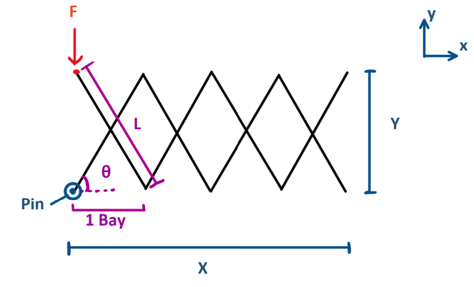
\includegraphics[width=0.5\linewidth]{Figures/systemDiagram.png}
    \caption{Scissor mechanism geometry and coordinate definition}
\end{figure}

\noindent
Notation: $s\theta \equiv \sin\theta$, $c\theta \equiv \cos\theta$, and $\nh{1},\nh{2}$ are the
body-frame unit vectors. The single generalized coordinate is $q=\theta$. $V$ denotes hinge-spring
potential energy; $\Vg$ denotes enclosed gas volume.
\section{Position Kinematics}

Center of mass of the first rod:
\begin{equation}
\vec{r}_1 = \tfrac{1}{2}L\ct\,\nh{1} + \tfrac{1}{2}L\st\,\nh{2}
\end{equation}

Center of mass of the second rod (offset by one full link):
\begin{equation}
\vec{r}_2 = L\cos\theta + \tfrac{1}{2}L\ct
\end{equation}

Generalizing to the $i$-th rod:
\begin{equation}
\vec{r}_i = \Big[(i-1)L\ct + \tfrac{1}{2}L\ct\Big]\nh{1} + \tfrac{1}{2}L\st\,\nh{2}
\label{eq:ri}
\end{equation}

\section{Velocity Kinematics}

Differentiating in time:
\begin{align}
\vec{v}_1 &= \Big[-\tfrac{1}{2}L\st\,\dth\Big]\nh{1} + \Big[\tfrac{1}{2}L\ct\,\dth\Big]\nh{2} \\[4pt]
\vec{v}_2 &= -L\st\,\dth - \tfrac{1}{2}L\st\,\dth = -\tfrac{3}{2}L\st\,\dth \\[4pt]
\vec{v}_i &= \Big(\tfrac{1}{2}-i\Big)L\st\,\dth\,\nh{1}
\label{eq:vi}
\end{align}

Check of the index coefficient in \eqref{eq:vi}:
\begin{equation}
\tfrac{1}{2}-1 = -\tfrac{1}{2},
\qquad
\tfrac{1}{2}-2 = -\tfrac{3}{2}
\end{equation}
which reproduces $\vec{v}_1$ and $\vec{v}_2$.

\subsection*{Index identity}

The squared coefficient that appears in the kinetic energy expands as
\begin{equation}
\Big(\tfrac{1}{2}-i\Big)^{2}
= \Big(\tfrac{1}{2}\Big)^{2} - i + i^{2}
= i(i-1) + \Big(\tfrac{1}{2}\Big)^{2}
= i(i-1) + \tfrac{1}{4}
\label{eq:idx}
\end{equation}

\section{Kinetic Energy}

The total kinetic energy splits by component group:
\begin{equation}
T = T_{\text{rods}} + T_{\text{supports}} + T_{\text{panels}}
\end{equation}

Summing translational and rotational contributions over the $n$ links:
\begin{equation}
T = \sum_{i=1}^{n}
\left[
\tfrac{1}{2}M_j\Big(\tfrac{1}{2}-i\Big)^{2}L^{2}s^{2}\theta\,\dth^{2}
+ \tfrac{1}{2}I_j\,\dth^{2}
\right]
\label{eq:T}
\end{equation}

Substituting the identity \eqref{eq:idx} into \eqref{eq:T}:
\begin{equation}
T = \sum_{i=1}^{n}
\left[
\tfrac{1}{2}M_j\,i(i-1)\,L^{2}s^{2}\theta\,\dth^{2}
+ \tfrac{1}{8}M_j L^{2}s^{2}\theta\,\dth^{2}
+ \tfrac{1}{2}I_j\,\dth^{2}
\right]
\label{eq:Texp}
\end{equation}

\section{Potential Energy — Hinge Springs}

Energy stored in the $N$ spring joints:
\begin{equation}
V = \tfrac{1}{2}k\theta^{2}\cdot N
\end{equation}



\section{Pressure Generalized Force}

\subsection*{Virtual work}

The gas exerts a traction $P\hat{n}$ on the wetted membrane, so under a virtual displacement
$\delta\vec{r}$ of that surface,
\begin{equation}
\delta W_p = \DP \oint_S \hat{n}\cdot\delta\vec{r}\,dA = \DP\,\delta \Vg,
\qquad \DP = P_{int}-P_{ext}
\end{equation}
since the surface integral is the first variation of enclosed volume. Specializing to $\delta \Vg =
(\partial \Vg/\partial\theta)\delta\theta$:
\begin{equation}
Q_p = \DP\,\frac{\partial \Vg}{\partial\theta}
\label{eq:Qp}
\end{equation}
On orbit $P_{ext}=0$ so $\DP = P_{int}$.

% \subsection*{Why the volume depends on $\theta$ at all}

% The tube is bonded to the members (rigid, inextensible arclength), so a naive model gives
% $\partial \Vg/\partial\theta = 0$ — bending a constant-arclength tube of circular cross-section
% changes nothing. The resolution: an inextensible membrane cannot hold a circular cross-section
% through a finite bend, so the section locally collapses at each kink, producing a volume deficit
% that is recovered as the kink straightens. The kinks are therefore the actuator.

\subsection*{Kink deviation angle}

At a kink the tube arrives along $(\ct,\st)$ and departs along $(\ct,-\st)$, so the deviation from
straight is
\begin{equation}
\beta = 2\theta, \qquad \frac{d\beta}{d\theta} = 2
\end{equation}
At $\theta=\pi/2$: $\beta=\pi$ (folded flat, stowed, max deficit). At $\theta=\theta_{min}$:
$\beta = 2\theta_{min}$ (kinks nearly open).

\subsection*{Volume function}

Writing volume as a straight-tube baseline less a deficit at each of $N_k$ kinks:
\begin{equation}
\Vg(\theta) = V_0 - N_k\,\Delta V(\beta) = V_0 - N_k\,\Delta V(2\theta)
\label{eq:Vfunc}
\end{equation}
with $V_0 = \pi R^2 s_{tube}$ ($R$ = inflated tube radius) and $\Delta V(0)=0$, increasing in $\beta$.

\subsection*{Kink moment}

Substituting \eqref{eq:Vfunc} into \eqref{eq:Qp} via the chain rule:
\begin{equation}
Q_p = \DP\,\frac{\partial \Vg}{\partial\theta}
= -2N_k\,\DP\,\frac{d\Delta V}{d\beta}\bigg|_{\beta=2\theta}
\end{equation}
Defining the kink moment
\begin{equation}
\Mk(\beta,\DP) \equiv \DP\,\frac{\partial \Delta V}{\partial\beta}
\qquad\Longrightarrow\qquad
\boxed{Q_p = -2N_k\,\Mk(2\theta,\DP)}
\label{eq:Qp_final}
\end{equation}
$\Mk>0$, so $Q_p<0$: pressure drives $\theta$ down from $\pi/2$ toward $\theta_{min}$, same sense
as the hinge springs. $\Mk$ appears in the same slot as $k(\theta-\theta_0)$. Essentially the pressurized tube
is a nonlinear torsional spring in parallel with the hinge springs.

\subsection*{Closure forms}

Dimensional scaling gives $\Mk = a\,\DP R^3 f'(\beta)$. Two candidate closures:
\begin{align}
\text{(C1) constant fold moment:}\quad & \Mk = a\,\DP\,R^{3} \\
\text{(C2) smooth vanishing fold:}\quad & \Mk = a\,\DP\,R^{3}\sin 2\theta
\end{align}
% (C2) predicts zero actuator moment at $\theta=\pi/2$ exactly (unstable symmetric fold) — the hinge
% springs must be sized to initiate motion regardless of closure choice. $f'(\beta)$ (equivalently $a$)
% is an empirical input, obtained from a single-kink or blocked-moment bench test.

\section{Lagrangian and Equation of Motion}

\begin{equation}
\mathcal{L} = T - V,
\qquad
H = T + V
\end{equation}

The forced Euler--Lagrange equation with $q=\theta$:
\begin{equation}
\frac{d}{dt}\!\left(\frac{\partial \mathcal{L}}{\partial \dot{q}}\right)
- \frac{\partial \mathcal{L}}{\partial q}
= Q_p + Q_F
\label{eq:EL}
\end{equation}

\subsection*{Momentum term}

\begin{equation}
\frac{\partial \mathcal{L}}{\partial \dth}
= M_j\,i(i-1)L^{2}s^{2}\theta\,\dth
+ \Big[I_j + \tfrac{1}{2}M_j L^{2}\Big]\dth
\end{equation}

\begin{equation}
\frac{d}{dt}\!\left(\frac{\partial \mathcal{L}}{\partial \dth}\right)
= M_j\,i(i-1)L^{2}s^{2}\theta\,\ddth
+ 2M_j\,i(i-1)L^{2}\st\ct\,\dth^{2}
+ \Big[I_j + \tfrac{1}{2}M_j L^{2}\Big]\ddth
\label{eq:ddt}
\end{equation}

\subsection*{Coordinate term}

\begin{equation}
\frac{\partial \mathcal{L}}{\partial \theta}
= M_j\,i(i-1)L^{2}\dth^{2}\,\st\ct - k\theta
\label{eq:dq}
\end{equation}

\subsection*{Assembled equation}

Substituting \eqref{eq:ddt}, \eqref{eq:dq}, and $Q_p$ from \eqref{eq:Qp_final} into \eqref{eq:EL},
with the two $\st\ct\,\dth^2$ terms combining ($2-1=1$), and moving $Q_p$ to the LHS alongside the
spring term (it is likewise a function of $\theta$ alone at fixed $\DP$):
\begin{equation}
\boxed{
\Big[M_j\,i(i-1)L^{2}s^{2}\theta + I_j + \tfrac{1}{2}M_j L^{2}\Big]\ddth
+ M_j\,i(i-1)L^{2}\st\ct\,\dth^{2}
+ k\theta
+ 2N_k\,\Mk(2\theta,\DP)
= Q_F
}
\end{equation}


\section{PHASE 1}

From $\theta = \pi/2$ till the system no longer experiences the moment singularity due to kinking, we
will rely solely on the hinged springs to generate enough force in the system. As such we have a
simplified version of the Lagrange with no pressure force ($Q_p = Q_F = 0$):

\begin{equation}
\underbrace{\Big[M_j\,i(i-1)L^{2}s^{2}\theta + I_j + \tfrac{1}{2}M_j L^{2}\Big]}_{I_{\text{eff}}(\theta)}\ddth
+ M_j\,i(i-1)L^{2}\st\ct\,\dth^{2}
+ N_s k\theta
= 0
\label{eq:phase1}
\end{equation}

This diff eq can be solved using \textbf{conservation of energy (first integral of motion)}, since the
system is scleronomic and unforced here: $H=T+V$ is conserved.
\begin{equation}
\tfrac{1}{2}I_{\text{eff}}(\theta)\,\dth^{2} + \tfrac{1}{2}N_s k\theta^{2} = E
\end{equation}

Assuming a desired duration of \emph{t}, starting from rest at $\theta(0)=\pi/2$, so
$E = \tfrac{1}{2}N_s k(\pi/2)^2$:
\begin{equation}
\dth = -\sqrt{\frac{N_s k\big[(\pi/2)^2 - \theta^2\big]}{I_{\text{eff}}(\theta)}}
\end{equation}
Integrating from stowage to the Phase 1 endpoint $\theta_1$:
\begin{equation}
t = \frac{1}{\sqrt{N_s k}}\int_{\theta_1}^{\pi/2} \sqrt{\frac{I_{\text{eff}}(\theta)}{(\pi/2)^2-\theta^2}}\;d\theta
\end{equation}

The required spring constant (based on all known mass parameters) is:
\begin{equation}
\boxed{
k = \frac{1}{N_s t^{2}}\left[\int_{\theta_1}^{\pi/2} \sqrt{\frac{I_{\text{eff}}(\theta)}{(\pi/2)^2-\theta^2}}\;d\theta\right]^{2}
}
\end{equation}

\section{PHASE 2}

Past $\theta_1$, kinking becomes reliable and the pressure generalized force $Q_p$ enters. 
\begin{equation}
I_{\text{eff}}(\theta)\,\ddth + M_j\,i(i-1)L^{2}\st\ct\,\dth^{2} + N_s k\theta + 2N_k M_{k0} = 0
\label{eq:phase2}
\end{equation}
where $M_{k0} \equiv M_k\big|_{C1}$ is the unknown constant kink moment to be solved for.

Because $M_{k0}$ is constant, $Q_p$ is still conservative: define an actuator potential referenced to
the Phase 1/2 boundary,
\begin{equation}
U_p(\theta) = 2N_k M_{k0}\,(\theta - \theta_1), \qquad U_p(\theta_1) = 0
\end{equation}

\subsection*{Boundary matching}

Continuity with Phase 1 fixes the initial condition of Phase 2 at $\theta_1$:
\begin{equation}
\dth_1 = -\sqrt{\frac{N_s k\big[(\pi/2)^2-\theta_1^{2}\big]}{I_{\text{eff}}(\theta_1)}}
\end{equation}

\subsection*{Energy conservation}

\begin{equation}
\tfrac{1}{2}I_{\text{eff}}(\theta)\,\dth^{2} + \tfrac{1}{2}N_s k\theta^{2} + 2N_k M_{k0}(\theta-\theta_1)
= \tfrac{1}{2}I_{\text{eff}}(\theta_1)\,\dth_1^{2} + \tfrac{1}{2}N_s k\theta_1^{2}
\end{equation}

Solving for $\dth$:
\begin{equation}
\dth = -\sqrt{\frac{I_{\text{eff}}(\theta_1)\dth_1^{2} + N_s k(\theta_1^{2}-\theta^{2}) - 4N_k M_{k0}(\theta-\theta_1)}{I_{\text{eff}}(\theta)}}
\end{equation}

Integrating to the full-deployment angle $\theta_{min}$, the desired Phase 2 duration $t_2$ implicitly
determines the required kink moment:
\begin{equation}
\boxed{
t_2 = \int_{\theta_{min}}^{\theta_1}
\sqrt{\frac{I_{\text{eff}}(\theta)}{I_{\text{eff}}(\theta_1)\dth_1^{2} + N_s k(\theta_1^{2}-\theta^{2}) - 4N_k M_{k0}(\theta-\theta_1)}}\;d\theta
}
\end{equation}

Unlike Phase 1, this does not invert cleanly for $M_{k0}$ (it sits inside the integrand as well as
scaling the whole bracket), so it must be solved numerically, e.g.\ root-find $M_{k0}$ so this integral equals the
target $t_2$.

% \subsection*{From $M_{k0}$ to pressure and tube geometry}

% With $M_{k0}$ fixed, the $C1$ closure gives one equation in two design unknowns:
% \begin{equation}
% M_{k0} = a\,\DP\,R^{3}
% \end{equation}
% $a$ (or the derating factor $\eta a$, Section 13 of the pressure derivation) comes from the bench test;
% $R$ is then a free design choice, with $\DP = M_{k0}/(aR^3)$ following directly, or vice versa if $\DP$
% is constrained instead by the supply hardware.
% % \section{External Generalized Force}

% \begin{equation}
% Q_F = \vec{F}\cdot\vec{\gamma} + \vec{M}\cdot\frac{\partial \vec{\omega}}{\partial \dot{q}}
% \end{equation}

% with the standard kinematic identity used to build the partial velocity $\vec{\gamma}$:
% \begin{equation}
% \frac{\partial \vec{r}}{\partial \theta} = \frac{\partial \dot{\vec{r}}}{\partial \dth}
% \end{equation}

% A configuration- and time-dependent panel load is written $F(A,t)$.

% \section{Supporting Relations}

% Double-angle identity used to collapse the $\st\ct$ products:
% \begin{equation}
% s2\theta = 2\,\st\,\ct
% \end{equation}

% Velocity and acceleration in a rotating reference frame:
% \begin{equation}
% \vec{v} = \vec{v}_{\text{ref}} + \vec{v}_{\text{loc}} + \vec{\omega}\times\vec{r}
% \end{equation}

% \begin{equation}
% \vec{a} = \vec{a}_{\text{ref}} + \vec{a}_{\text{loc}}
% + \underbrace{2\,\vec{\omega}\times\vec{v}_{\text{loc}}}_{\text{Coriolis}}
% + \underbrace{\vec{\alpha}\times\vec{r}}_{a_t}
% + \underbrace{\vec{\omega}\times(\vec{\omega}\times\vec{r})}_{a_n}
% \end{equation}

\end{document}